\documentclass{standalone}
\usepackage{tikz}

\begin{document}

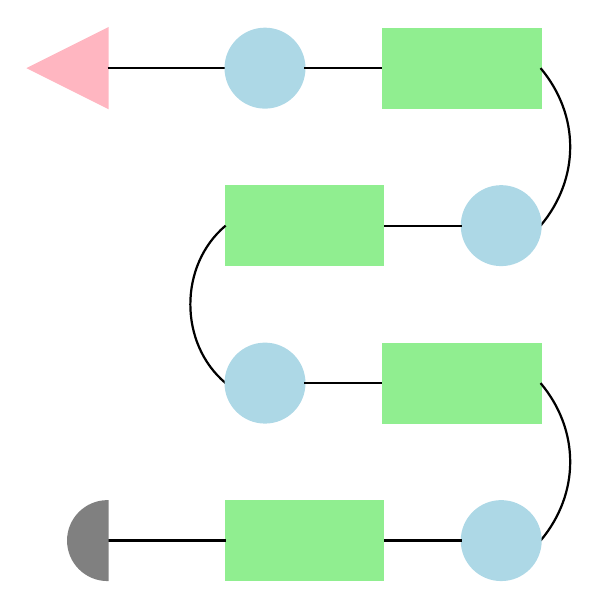
\begin{tikzpicture}

    % Define colors
    \definecolor{pastelblue}{RGB}{173,216,230}
    \definecolor{pastelyellow}{RGB}{255,255,204}
    \definecolor{pastelgreen}{RGB}{144,238,144}
    \definecolor{pastelred}{RGB}{255,182,193}


    \filldraw[pastelred, thick] (-3,0) -- (-2,0.5) -- (-2,-0.5) -- cycle;
    \draw[thick] (-2,0) to (0,0);

    \filldraw[pastelblue, thick] (0,0) circle(0.5);
    \draw[thick] (0.5,0) to (1.5,0);
    \filldraw[pastelgreen, thick] (1.5,0.5) rectangle (3.5,-0.5);

    %-------------
    \draw[thick] (3.5,0) to[out=-50,in=50] (3.5,-2);
    %-------------
    % Second row

    \filldraw[pastelblue, thick] (3,-2) circle(0.5);
    \draw[thick] (2.5,-2) to (1.5,-2);
    \filldraw[pastelgreen, thick] (-0.5,-1.5) rectangle (1.5,-2.5);

    %-------------
    \draw[thick] (-0.5,-2) to[out=-140,in=140] (-0.5,-4);
    %-------------
    % Third row

    \filldraw[pastelblue, thick] (0,-4) circle(0.5);
    \draw[thick] (0.5,-4) to (1.5,-4);
    \filldraw[pastelgreen, thick] (1.5,-3.5) rectangle (3.5,-4.5);


    %-------------
    \draw[thick] (3.5,-4) to[out=-50,in=50] (3.5,-6);
    %-------------
    % Fourth row

    \filldraw[pastelblue, thick] (3,-6) circle(0.5);
    \draw[thick] (1.5,-6) to (2.5,-6);
    \filldraw[pastelgreen, thick] (-0.5,-5.5) rectangle (1.5,-6.5);
    
    \draw[thick] (-2,-6) to (-0.5,-6);
    \filldraw[gray, thick] (-2,-5.5) arc[start angle=90,end angle=270,radius=0.5] -- cycle;

\end{tikzpicture}

\end{document}
